\documentclass{article}
\usepackage{graphicx}
\usepackage{pgfplots}

\title{2D Blocks Report}
\author{CHAPUIS Julien}
\date{\today}

\begin{document}
\section{Grayscale Conversion}
The grayscale conversion is parallelized using 2D blocks. Each CUDA thread processes one pixel, and thread indices are calculated based on their 2D coordinates:

\[
x = \text{threadIdx.x} + \text{blockIdx.x} \times \text{blockDim.x}
\]
\[
y = \text{threadIdx.y} + \text{blockIdx.y} \times \text{blockDim.y}
\]

The block sizes are (8x8), (16x16), and (32x32).

\section{Performance Results}

\begin{table}[h]
\centering
\begin{tabular}{|c|c|}
\hline
\textbf{Block Size} & \textbf{GPU Time (s)} \\
\hline
(8, 8)   & 0.341955 \\
(16, 16) & 0.005590 \\
(32, 32) & 0.002057 \\
\hline
\end{tabular}
\caption{GPU Execution Time for Different Block Sizes}
\label{table:performance}
\end{table}

We can see that the more blocks we use, the faster it is. This is due to the fact that the more blocks we use, the more threads we can run in parallel. This is shown in the speedup plot in Figure \ref{fig:speedup_plot}.

\begin{figure}[h]
\centering
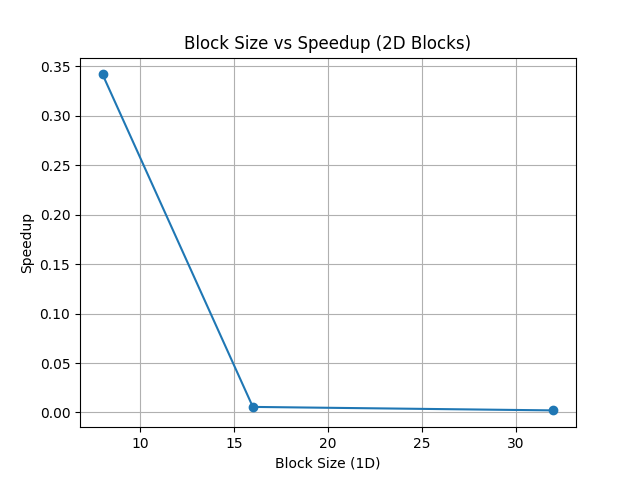
\includegraphics[width=0.7\textwidth]{block_size_vs_speedup.png}
\caption{Block Size vs Speedup}
\label{fig:speedup_plot}
\end{figure}


\end{document}



\end{document}